\chapter{Introduction}\label{ch:Introduction}
World War I, a time of harsh conflict and battle, provided an example of how
cooperation need not evolve from friendship. Indeed,~\cite{Axelrod1984a} states
that small units of common soldiers on the Western Front were able to execute a
``live and let live'' system, even against the will of the officers. They knew
that ``if the British shelled the Germans, the Germans replied; and the damage
was equal'' (quoted from~\cite{Cobb1916} as given in~\cite{Axelrod1984a}).
Moreover, this was achieved without a direct truce as officers forbade it. The
analysis of such circumstances, and other situations involving choice, is
covered by an area of mathematics entitled \textit{game theory}.

According to~\cite{Dictionary2013}, \textit{game theory} is the study of interactive
decision making and the development of
strategies through mathematics. It analyses and gives
methods for predicting the choices made by players (those making a decision),
whilst also suggesting ways to improve their
`outcome'~\cite{maschler_solan_zamir_2013}. Here, the abstract notion of utility
is the outcome players wish to maximise. For further information on the topic of
utility theory, readers are referred to Chapter 2
in~\cite{maschler_solan_zamir_2013} for a detailed discussion or Section
1.3 in~\cite{Webb2007} for a more introductory explanation. 

One of the earliest pioneers of game theory is mathematician, John von Neumann
who, along with economist Oskar Morgenstern, published \textit{The Theory of
Games and Economic Behaviour} in 1944~\cite{maschler_solan_zamir_2013}. This
book~\cite{von2007theory} discusses the theory, developed in 1928 and 1940, by von Neumann,
regarding ``games of strategy'' and its applications within the subject of
economics. Following this, several advancements have been
made in the area including, most notably, John Nash's papers on the
consequently named
Nash Equilibria in 1950-51~\cite{nash1950equilibrium,nash1951non}. Due to the
``context-free mathematical toolbox''~\cite{maschler_solan_zamir_2013} nature of
this subject, it has been applied to many areas, from
networks~\cite{liang2012game, 1593279} to biology~\cite{adeoye2012application, chen2009robust}. 

In this project, the main focus is a
class of theorems within game theory, known as ``Folk Theorems''. These ideas
assist in the analysis of long-term behaviour and evolution of cooperative
strategies. In particular, the theory will be applied to the game of a
Prisoner's Dilemma which is introduced in subsequent sections. The structure of
this report is as follows: Chapter~\ref{ch:Lit_Review} provides a literature review
on the topic of folk theorems, before Chapter~\ref{ch:Methods} discusses the
development of a large experiment regarding these notions in the Prisoner's
Dilemma. Chapter~\ref{ch:Analysis} analyses the results obtained
whilst Chapter~\ref{ch:Conclusions} provides the conclusions and recommendations for
further study. However, first, the remainder of Chapter~\ref{ch:Introduction} is dedicated
to the key definitions and theorems required for a study in game theory.

Unless stated otherwise, the definitions and notation in this chapter have been
adapted from~\cite{maschler_solan_zamir_2013}.

\section{An Introduction to Games}\label{sec:An_Intro_to_Games}
Consider the following scenario:

\begin{center}
    Two convicts have been accused of an illegal act. Each of these prisoners,
    separately, have to decide whether to reveal information (defect) or stay
    silent (cooperate). If they both cooperate then the convicts are given a
    short sentence whereas if they both defect then a medium sentence awaits.
    However, in the situation of one cooperation and one defection, the prisoner
    who cooperated has the consequence of a long term sentence, whilst the other
    is given a deal~\cite{Knight2017, maschler_solan_zamir_2013}.
\end{center}

This is one of the standard games in game theory known as the Prisoner's
Dilemma (PD). It has four distinct outcomes, for the given two player version,
which can be viewed in Table~\ref{tab:PD_outcomes}. Note, following the standard
literature, cooperation and defection is indicated by \(C\) and \(D\), respectively.

\begin{table}
    \centering
    \begin{tabular}{c|c}
        \(C, C\) & \(C, D\) \\
        \midrule
        \(D, C\) & \(D, D\) \\
    \end{tabular}
    \caption{Outcomes for a game of the Prisoner's Dilemma.}\label{tab:PD_outcomes}
\end{table}

More formally, the game can be represented as the following matrix:
\begin{equation}\label{eqn:PDMatrix}
    \kbordermatrix{
        \mbox{ } & C & D\\ 
        C & (3, 3) (R, R) & (0, 5) (S, T)\\ 
        D & (5, 0) (T, S) & (1, 1) (P, P)
    }
\end{equation}
where each coordinate \((a, b)\) in the table represents the utility values
obtained for each player, where \(a\) is the utility value obtained by the row
player and \(b\) is the utility gained by the column player. These utility
values (payoffs)\footnote{`Utility' is referred to as a player's `payoff'
throughout the remainder of this report.} are as given
in~\cite{axelrod1980effective} and
used throughout this project. In general, the PD payoffs are constrained by the
two conditions:

\begin{equation}\label{eqn:PD_1}
    T > R > P > S
\end{equation}
and
\begin{equation}\label{eqn:PD_2}
    2R > T + S
\end{equation}

where~(\ref{eqn:PD_1}) ensures that \(D\) is preferable to \(C\) and
yet~(\ref{eqn:PD_2}) ensures that mutual \(C\) is
best~\cite{Knight2019,Press2012}. The matrix given in~(\ref{eqn:PDMatrix}) is
known as a \textit{normal form} representation of the game.

\begin{definition}
    In general a \textit{normal form} or \textit{strategic form} game is defined
    by an ordered triple \(G = (N, {(S_i)}_{i \in N}, {(u_i)}_{i \in N})\), where:
    \begin{itemize}
        \item \(N = \{1, 2,\ldots, n\} \) is a finite set of players;
        \item \(S = S_1 \times S_2, \times \cdots \times S_n\) is the set of
        strategies for all players in which each vector \({(S_i)}_{i \in N}\) is
        the set of strategies for player \(i\)\footnote{Since the game of the PD has a finite strategy set for each player \(S_i=\{\text{C},
        \text{D}\} (i = 1, 2, \ldots, n)\), in this project only finite
        strategy spaces are considered.}; and
        \item \(u_i : S \to \mathbb{R}\) is a payoff function which associates each
        strategy vector, \(s = {(s_i)}_{i \in N}\), with a utility
        \(u_i(i \in N)\).
    \end{itemize}
\end{definition}

Yet another way of representing this game is as a pair of matrices, \(A, B\),
defined as follows:
\begin{equation}
    A = 
    \begin{pmatrix}
       3 & 0\\
       5 & 1\\ 
    \end{pmatrix}
    \text{ and } B = A^{T} =
    \begin{pmatrix}
        3 & 5\\
        0 & 1\\
    \end{pmatrix}
\end{equation}
This way of defining games allows for the use of linear algebraic expressions in
the calculation of utilities (see Section~\ref{sec:NE_for_Normal_Form_Games}).

Before continuing the discussion into the key notions of game theory, it needs
to be highlighted that there is an important assumption, which is central to
most studies of game theory, entitled \textit{Common Knowledge of Rationality}.
This, more formally, is a recurring list of beliefs which claim:
    \begin{itemize}
        \item The players are rational;
        \item All players know that the other players are rational;
        \item All players know that the other players know that they are 
        rational; 
        \item etc.    
    \end{itemize}
Assuming Common Knowledge of Rationality allows for the prediction of rational
behaviour through a process known as \textit{rationalisation}
~\cite{Knight2019}. See Section 4.5 in~\cite{maschler_solan_zamir_2013} for an
alternative explanation of this assumption. 

Thus far, only the pure strategies, \(S_{i}=\{C, D\} \), have
been discussed, hence the notion of a probability distribution over \(S_{i}\) is
now introduced, giving the so-called \textit{mixed strategies}.

\begin{definition}
   Let \(G=(N, {(S_{i})}_{i \in N}, {(u_{i})}_{i \in N})\) be a game, then a \textit{mixed strategy} for player \(i\) is a
probability distribution over their strategy set \(S_{i}\). The set of mixed
strategies for player \(i\) is defined by 
\begin{equation}
    \Sigma_{i} = \left \{ \sigma_{i} : S_{i} \to [0, 1] \mid \sum_{s_{i} \in S_{i}}{\sigma_
{i}(s_{i})} = 1 \right \}. 
\end{equation}
\end{definition}

Hence, observe that the pure
strategies are specific cases of mixed strategies, with \(\sigma_{i} = (1, 0)\)
for cooperation and \(\sigma_{i} = (0, 1)\) for defection, in the PD\@.

This leads onto the following definition of a \textit{mixed extension} for a
game.

\newpage
\begin{definition}
    Let \(G\) be a finite normal form game as above, with \(S = S_{1} \times
S_{2} \times \cdots \times S_{n}\) defining the pure strategy vector set and
each pure strategy set, \(S_{i}\) being non-empty and finite. Then the
\textit{mixed extension} of \(G\) is denoted by
\begin{equation}
    \Gamma = (N, {(\Sigma_{i})}_{i \in N}, {(U_{i})}_{i \in N}), 
\end{equation}
and is the game in which, \(\Sigma_{i}\) is the \(i\)th player's strategy set
and \(U_{i} : \Sigma \to \mathbb{R}\) is the corresponding payoff function,
where each \(\sigma = (\sigma_{1}, \sigma_{2}, \ldots, \sigma_{n}) \in \Sigma =
\Sigma_{1} \times \Sigma_{2} \times \cdots \times \Sigma_{n}\) is mapped to the
payoff:
\begin{equation}\label{eqn:mixed_payoff_function}
    U_{i} = \mathbb{E}_{\sigma}(u_{i}(\sigma)) = \sum_{(s_{1}, s_{2}, \ldots, s_
    {n}) \in S}{u_{i}(s_{1}, s_{2}, \ldots, s_{n})\sigma_{1}(s_{1})\sigma_{2}(s_
    {2})\cdots\sigma_{n}(s_{n})} 
\end{equation}
for all players \(i \in N\).
\end{definition}

\section{Nash Equilibrium for Normal Form Games}\label{sec:NE_for_Normal_Form_Games}
As mentioned above, mathematician, John Nash, introduced the concept of an
equilibrium point and proved the existence of mixed strategy Nash Equilibria in
all finite games. These notions are central to the study of game
theory~\cite{maschler_solan_zamir_2013} and hence, in this section, Nash's
concepts will be defined and proved in detail.

Firstly, the idea of a \textit{best response} is introduced.
\begin{definition}
    For a game \(G=(N, {(S_{i})}_{i \in N}, {(u_{i})}_{i \in N})\), the strategy,
\(s_{i}\), of the \(i\)th player is considered a \textit{best response} to the
strategy vector \(s_{-i}\) if \(u_{i}(s_{i}, s_{-i}) = \max_{t_{i} \in
S_{i}}u_{i}(t_{i}, s_{-i})\).
\end{definition}

This leads onto the main definition of the section.
\begin{definition}\label{def:NE}
    Given a game \(G=(N, {(S_{i})}_{i \in N}, {(u_{i})}_{i \in N})\) and its
    mixed extension, \(\Gamma \), the vector of
    strategies \(\sigma^{*} = (\sigma_{1}^{*}, \sigma_{2}^{*}, \ldots, \sigma_{n}^{*})\) is a
    \textit{Nash equilibrium} if, for all players \(i \in N\), \(\sigma_{i}^{*}\) is 
    a best response to \(\sigma_{-i}^{*} \in N\).
\end{definition}

In other words, \(\sigma^{*}\) is a Nash equilibrium if and only if no player has any
reason to deviate from their current strategy \(\sigma_{i}^{*}\).

The following observation is highlighted as an example.

\begin{center}
    \textbf{The strategy pair \((D, D)\), is the unique Nash equilibrium 
    for the PD, with a payoff value of 1 for each player.}
\end{center}

Assume the row player uses the following mixed strategy, \(\sigma_{r} = (x,
1-x)\), that is, the probability of cooperating is \(x\) and the probability of
defecting is \(1-x\). Similarly, assume the column player has 
the strategy, \(\sigma_{c} = (y, 1-y)\). The payoff obtained for the row and column player, respectively, is then:
\[
    A\sigma_{c}^T = \begin{pmatrix}
        3 & 0 \\
        5 & 1
    \end{pmatrix} \begin{pmatrix}
        y \\
        1-y
    \end{pmatrix} = \begin{pmatrix}
        3y \\
        4y + 1
    \end{pmatrix},
\]
\[
    \sigma_{r}B = \begin{pmatrix}
        x & 1-x
    \end{pmatrix} \begin{pmatrix}
        3 & 5 \\
        0 & 1        
    \end{pmatrix}  = \begin{pmatrix}
        3x & 4x + 1
    \end{pmatrix}.
\]

Plotting these gives the graphs as seen in Figure~\ref{fig:mixed_strategy_PD}.

\begin{figure}
    \centering
    \begin{subfigure}{0.45\textwidth}
        \centering
        \includegraphics[width=\textwidth]{{pd-row-payoff}}
    \end{subfigure}
    \begin{subfigure}{0.45\textwidth}
        \centering
        \includegraphics[width=\textwidth]{{pd-col-payoff}}
    \end{subfigure}
    \caption{Graphs to show the row and column players' payoffs against a 
    mixed strategy.}\label{fig:mixed_strategy_PD}
\end{figure}

From Figure~\ref{fig:mixed_strategy_PD} it is clear that, regardless of the
strategy played by the opponent, defection is indeed the only rational move. Thus, the players have no incentive to deviate if and only if both
play the strategy \(\sigma=(0, 1)\), that is, defection for every one-shot game
of the PD\@.

This next result is taken from~\cite{nash1951non}, Nash's second paper on
equilibria in games. The notion obtained here is fundamental to many areas of
game theory, including the folk theorems.

\begin{theorem}\label{thm:Nash}
    Every finite game has an equilibrium point.
\end{theorem}

The proof of Theorem~\ref{thm:Nash} includes the use of a \textit{fixed point
theorem}. Thus, a short sub-section regarding one such result is given for
completeness, before providing a formal proof of Theorem~\ref{thm:Nash}.

\subsection{Brouwer's Fixed Point Theorem}\label{subsec:Brouwer_thm}
Brouwer's Fixed Point Theorem is a result from the field of topology. Named
after the Dutch mathematician, L.E.J. Brouwer, it was proven in
1912~\cite{Carlson2016}. However, before stating this notion, a few conditions
regarding the properties of sets are recalled. 

The following three definitions appear as 
in~\cite{Barile,Weissteina,Weisstein}
for Definitions~\ref{def:open_cover},~\ref{def:compact}, and~\ref{def:convex}, respectively.

\begin{definition}\label{def:convex}
    A set \(X \subseteq \mathbb{R}^{d}\) is called \textit{convex} if it
    contains all line segments connecting any two points \({x}_{1},
    {x}_{2} \in X\).
\end{definition}

\begin{definition}\label{def:open_cover}
    An \textit{open cover} of a set \(S \subset X\), a topological space, is a
    collection of open sets \(A_{1}, A_{2}, \ldots \subset X\) such that
    \(A_{1} \cup A_{2} \cup \ldots \supset S\), that is, the union of the open
    sets contain S.
\end{definition}

\begin{definition}\label{def:compact}
    A subset \(S \subseteq X\), a topological space, is called \textit{compact}
    if, for each open cover of \(S\), there is a finite sub-cover of S.
\end{definition}

The presentation of Brouwer's Fixed Point Theorem is now given as 
in~\cite{maschler_solan_zamir_2013}.

\begin{theorem}\label{thm:Brouwer}
    Let \(X \subseteq \mathbb{R}^{n}\) be a non-empty convex and compact
    set, then each continuous function \(f : X \to X\) has a fixed point.  
\end{theorem}

In other words if \(X\) and \(f\) satisfy the conditions given above then there
exists a point \(x \in X\) such that \(f(x) = x\). 

Since this project is regarding game theory, rather than topology, the proof to
the above theorem is omitted. However, the interested reader is referred
to~\cite{Henle1979} for an in-depth consideration into the theory of topology.

\subsection{Proof of Nash's Theorem}\label{subsec:Nash_Proof}
The proof provided is adapted from the original, as presented
in~\cite{nash1951non}, with extra notes from~\cite{maschler_solan_zamir_2013}.
According to~\cite{maschler_solan_zamir_2013}, the general idea is to
define a function, which satisfies the conditions required
for Theorem~\ref{thm:Brouwer}, by using the payoff functions on the set of mixed
strategies. Then, through identifying
each equilibrium point with a fixed point of the function, the required result 
is obtained.

Firstly, a brief restatement of the notation needed is provided for clarity.
Let \(G=(N, {(S_{i})}_{i \in N}, {(u_{i})}_{i \in N})\) be a finite game with
mixed extension \(\Gamma=(N, {(\Sigma_{i})}_{i \in N}, {(U_{i})}_{i \in N})\).
Here, \(N = \{1, \ldots, n\} \) denotes the set of players; \(S = S_{1} \times S_{2} \times
\ldots \times S_{n}\) is the set of pure strategies for all players, with
\({(S_i)}_{i \in N}\) the pure strategy set for player i; \(\Sigma \) is
defined similarly but relating to mixed strategies; and \(U_{i}: \Sigma \to
\mathbb{R}\) are the payoff functions as given in~(\ref{eqn:mixed_payoff_function}).

\begin{proof}
    Let \(\sigma = (\sigma_{1}, \sigma_{2}, \ldots, \sigma_{n})\) be a tuple of
    mixed strategies and \(U_{i,t}(\sigma)\) be the \(i\)th player's payoff if
    they changed to their \(s_{i}^{t}\)th pure strategy and all other players
    continue to use their mixed strategy.
    Now, define function \(f: \Sigma \to [0, \infty)\) such that 
    \begin{equation}
        f_{i,t}(\sigma) = \max{(0, U_{i,t}(\sigma)-U_{i}(\sigma))}
    \end{equation}
    and also let 
    \begin{equation}
        \sigma_{i}^{\prime} = \frac{ \sigma_{i}+\sum_{t}{f_{i,t}(\sigma)s_{i}^{t}} }{ 1+\sum_{t}{f_{i,t}(\sigma)} }
    \end{equation}
    be a modification of each \(\sigma_{i} \in \sigma \), with \(\sigma^{\prime}
    = (\sigma_{1}^{\prime}, \sigma_{2}^{\prime}, \ldots, \sigma_{n}^{\prime})\).
    In words, this modification increases the proportion of the pure strategy
    \(s_{i}^{t}\) used in \(\sigma_{i}\) if the payoff gained by the \(i\)th player is
    larger when they replace their mixed strategy by \(s_{i}^{t}\). Else, it remains the
    same if doing this decreases their payoff as \(f_{i,t}(\sigma)=0\) in this
    case. Note, the denominator ensures that the ending vector is still a
    probability distribution by standardising.

    The aim is to apply Theorem~\ref{thm:Brouwer} to the mapping \(T: \sigma \to
    \sigma^{\prime}\) and show that its fixed points correspond to Nash
    equilibria. Thus, firstly compactness and convexity of the set \(\Sigma \)
    is shown along with continuity of the function \(f\). 
    
    \textbf{Claim 1: The set \(\Sigma \) is compact and convex.}
    Observe that each \(\sigma_{i}\) can be represented by a point in a simplex
    in a real vector space with the vertices given by the pure strategies,
    \(s_{i}^{t}\). Therefore, it follows that the set \(\Sigma_{i}\) is convex
    and compact. Using the result, \textit{If \(A \subseteq \mathbb{R}^{n}\) and
    \(B \subseteq \mathbb{R}^{m}\) are convex compact sets then the set \(A
    \times B\) is a convex compact subset of \(\mathbb{R}^{n+m}\)} (highlighted in~\cite{maschler_solan_zamir_2013}), gives the convexity and
    compactness of the set \(\Sigma \), the cross product of all
    \(\Sigma_{i}\)s. 
    
    \textbf{Claim 2: The function \(f\) is continuous.}
    The continuity of the function \(f\) depends upon the continuity of the
    payoff functions \(U_{i}\). As given in~\cite{maschler_solan_zamir_2013},
    this is shown by first proving that the \(U_{i}\) are multilinear functions
    in the variables \({(\sigma_{i})}_{i \in N}\) and then applying the fact
    that any multilinear function over \(\Sigma \) is a continuous
    function\footnote{For a detailed consideration of the continuity of the
    payoff functions see~\cite{maschler_solan_zamir_2013}, pages
    148--149.}. The result then follows.

    Hence, by Theorem~\ref{thm:Brouwer}, the mapping \(T\) must have at least
    one fixed point. The proof is concluded by showing that any fixed points of
    \(T\) are Nash equilibria and vice versa. 

    \textbf{Claim 3: Any fixed point of \(T\) is a Nash equilibrium.}
    Suppose \(\sigma \) is such that \(T(\sigma) = \sigma \). Then the
    proportion of \(s_{i}^{t}\) used in the mixed strategy \(\sigma_{i}\) must
    not be altered by \(T\). Therefore, in \(\sigma_{i}^{\prime}\), the sum
    \(\sum_{t}{f_{i,t}(\sigma)}\) in the denominator must equal zero, otherwise the total sum of the denominator will be greater than one,
    decreasing the proportion of \(s_{i}^{t}\). This implies that for all pure
    strategies \(s_{i}^{q}\), \(f_{i,q}(\sigma)=0\). That is, player \(i\) can not
    improve their payoff by adopting any of the pure strategies. Note, this is
    true for all \(i\) and \(s_{i}^{q}\) by definition of \(T(\sigma) = \sigma
    \) and thus no player is able to improve their payoff. By Definition~\ref{def:NE},
    this is exactly the conditions of a Nash equilibrium.

    \textbf{Claim 4: Any Nash equilibrium is a fixed point of \(T\).}
    Assume \(\sigma \) is a Nash equilibrium. Then, by definition, it must
    be that \(f_{i,q}(\sigma)=0\) for all pure strategies \(q\) for all players,
    \(i \in N\). Note, if \(f_{i,q}(\sigma) \ne 0\), then the
    \(i\)th player would benefit from changing their strategy to the pure
    strategy \(s_{i}^{q}\), which violates the condition for a Nash equilibrium.
    From this it follows that \(T(\sigma) = \sigma \), that is, \(\sigma \) is a
    fixed point of \(T\). This concludes the proof.
\end{proof}

\section{Repeated Games}\label{sec:Repeated_Games}
The folk theorems studied in this project are a consequence of games which are
repeated several times. Indeed, repeated games provide more
insight into how and why cooperation can evolve. Moreover, there are cases in
which further equilibria become supported when compared to the one-shot
equivalent. It could also be argued that repeated games provide more realistic
results regarding interactions, since the majority of situations are faced on a
regular basis. Thus, before discussing the
main statements of the study, the theory of both finitely and infinitely
repeated games is presented.

Firstly, a couple of alterations to the terminology used in
previous sections is redefined, to be consistent with the
literature. The notion of a `game' will become known as a
\textit{stage game} to highlight the fact that a one-off game is being
considered. Also, what was defined previously as a `strategy' will now be
referred to as an \textit{action} to differentiate it from a strategy of a
repeated game, see Section~\ref{subsec:Finite_Repeated_Games}.

\subsection{Finite Repeated Games}\label{subsec:Finite_Repeated_Games}
According to~\cite{Knight2017}, a \textit{\(T\)-stage repeated game}, \(T <
\infty \) is when the stage game, \(G\), is played \(T\) times, over discrete
time intervals. Each player has a strategy based on previous `rounds' of
the game and the payoff of a repeated game is calculated as the total sum of the
stage game payoffs.

Prior to giving a formal description of a strategy in a repeated game, the idea
of \textit{history}, within the context of repeated games, is provided.

\begin{definition}\label{def:history}
    The \textit{history}, \(H(t)\) of a repeated game is the knowledge of
    previous actions of all players up until the \(t\)th stage game, assumed to
    be known by all players. Note that, when \(t=0\), \(H(0) =
\underbrace{(\emptyset, \emptyset, \ldots, \emptyset)}_{N \text{times}}\), since
no stage games have yet been played.
\end{definition}

\begin{definition}
    As given in~\cite{Knight2019,maschler_solan_zamir_2013}, a
    \textit{strategy} of a \(T\)-stage repeated
    game is defined to be a mapping from the complete history so far to an
    action of the stage game, that is 
    \begin{equation}
        \tau_{i} : \bigcup_{t = 0}^{T-1}{H(t)} \to a_{i}.
    \end{equation}    
\end{definition}

Here, \(H(t)\) is the history of play as defined in Definition~\ref{def:history} and
\(a_{i}\) is the \(i\)th player's action of the stage game. 

Consider, for example, the environment in which the stage game PD is repeated each time. This is known as the \textit{Iterated Prisoner's
Dilemma} (IPD) and has been a popular topic of research for many
years\footnote{The interested reader is referred to the following papers~\cite{Glynatsi2019,Jurisic2012,ORiordan2001} for
good reviews regarding the IPD.}. Note that the objective
here is to maximise payoff. The player: 
\begin{center}
    \textit{No matter what my opponents play, I will always defect},
\end{center}
commonly known as the `Defector' has the following strategy mapping:
\begin{equation}
    \tau_{i} : \bigcup_{t = 0}^{T-1}{H(t)} \to a_{i},    
\end{equation}
where \(a_{i}=D\) for all time periods \(\tau \ge 0\). Other common IPD
strategies include: 
\begin{itemize}
    \item Cooperator --- \textit{No matter what my opponents play, I will always
    cooperate};
    \item Random --- \textit{I will either cooperate or defect with a probability of
    50\%}; and
    \item Tit For Tat --- \textit{I will start by cooperating but then will 
    duplicate the most recent decision of my opponent.}
\end{itemize}

Figure~\ref{fig:2-stage_payoff_plot} shows the possible payoffs obtained in
a 2-stage repeated IPD with two players.

\begin{figure}
    \centering
    \resizebox{0.5\textwidth}{!}{\begin{tikzpicture}
    \draw[->] (0, 0) -- (11, 0);
    \draw[->] (0, 0) -- (0, 11);
    \foreach \x in {0,2,4,6,8,10}
        \draw (\x cm,2pt) -- (\x cm,-1pt) node[anchor=north] {$\x$};
    \foreach \y in {0,2,4,6,8,10}
        \draw (2pt,\y cm) -- (-1pt,\y cm) node[anchor=east] {$\y$};
    \filldraw [blue] (2, 2) circle (2pt);
    \filldraw [blue] (0, 10) circle (2pt);
    \filldraw [blue] (10, 0) circle (2pt);
    \filldraw [blue] (6, 6) circle (2pt);
    \filldraw [blue] (3, 8) circle (2pt);
    \filldraw [blue] (8, 3) circle (2pt);
    \filldraw [blue] (1, 6) circle (2pt);
    \filldraw [blue] (6, 1) circle (2pt);
    \filldraw [blue] (4, 4) circle (2pt);
\end{tikzpicture} }
    \caption{A plot to show the possible payoffs of the game between two players in which the PD is repeated twice.}\label{fig:2-stage_payoff_plot}
\end{figure}

Now, a discussion on Nash equilibria in repeated games is provided. It can be
proven that there exist many equilibria in repeated
games~\cite{Friedman1971}. The next result,
adapted from~\cite{Knight2019,maschler_solan_zamir_2013} guarantees at least
one.

\newpage
\begin{theorem}\label{thm:seq_of_stage_NE} 
    Consider a \(T\)-stage repeated game with \(G=(N, {(S_{i})}_{i \in N},
    {(u_{i})}_{i \in N})\) as the stage game, \(0 < T < \infty \). Define by
    \( {\sigma}^{*} = (\sigma_{1}^{*}, \sigma_{2}^{*}, \ldots,
    \sigma_{n}^{*})\), a stage Nash equilibrium of \(G\). Then the sequence in
    which \({\sigma}^{*}\) is continuously played is a Nash equilibrium of the
    \(T\)-stage repeated game.
\end{theorem}

\begin{proof}
    Since \( \sigma^{*} \) is a stage Nash equilibrium, it is, in particular,
    a Nash equilibrium of the \(T\)th stage game. Thus, no player has any reason
    to deviate here. However, \( \sigma^{*} \) was also played at the
    \((T-1)\)th stage, meaning there is still no reason to deviate.
    Therefore, continuing via backwards induction gives the required result.
\end{proof}

Hence, for the \(T\)-stage IPD, all players executing the Defector strategy
yields a Nash equilibrium. However, it could be argued that this does not
explain why cooperation evolves in many situations.

\subsection{Infinite Repeated Games}\label{subsec:Infinite_Repeated_Games}
This section discusses the case when \(T \to \infty \) and results linked to
\textit{infinitely repeated games}. These provide a more realistic framework for
analysing behaviours. 

\newpage
\subsubsection{Extensive Form Games}\label{subsubsec:Extensive_Form_Games}
The Folk Theorem discussed in Section~\ref{sec:Folk_Thm}
considers a stronger refinement of Nash equilibria, for repeated games, known as
\textit{subgame perfect equilibria}. In order to fully understand this notion, a
new representation of games is introduced.

\begin{definition}
   An \textit{extensive form game} is given by the ordered vector
\(\Gamma = (N, V, E, x_{0}, {(V_{i})}_{i \in N}, O, u)\)
where \(N=\{1, 2, \ldots, n\} \) is a finite set of players; \((V, E, x_{0})\)
is a \textit{game tree}\footnote{The triple \((V, E, x_{0})\) is defined as a
\textit{tree} if the set of vertices, \(V\), and the set of edges, \(E\), create
a \textit{directed graph}, that is, each element in \(E\) is an ordered tuple.
The root, or starting node, of the graph is represented by \(x_{0}\)};
\({(V_{i})}_{i \in N}\) is a partition of the set \(V \setminus L\), where \(L\)
is the set of all
leaves, or terminal points, of the game tree; \(O\) is the set of outcomes for
the game; and \(u\) is a function which maps each leaf in \(L\) to an outcome 
in \(O\). 
\end{definition}

This leads on to the following definition, adapted from~\cite{Webb2007}.

\begin{definition}
    A player's \textit{information set} is a subset of the nodes in a game tree
    where:
    \begin{itemize}
        \item Only the player concerned is deciding;
        \item This player is not aware of which node has been reached, except
        that it is definitely one of the elements found in this set.
    \end{itemize}     
\end{definition}

In Figure~\ref{fig:PD_game_tree}, the extensive form representation of the
PD is provided. Here, only two players are considered and
any information sets are represented by a dashed line. Any normal form
game can be represented as an extensive form game. 

\begin{figure}
    \centering
    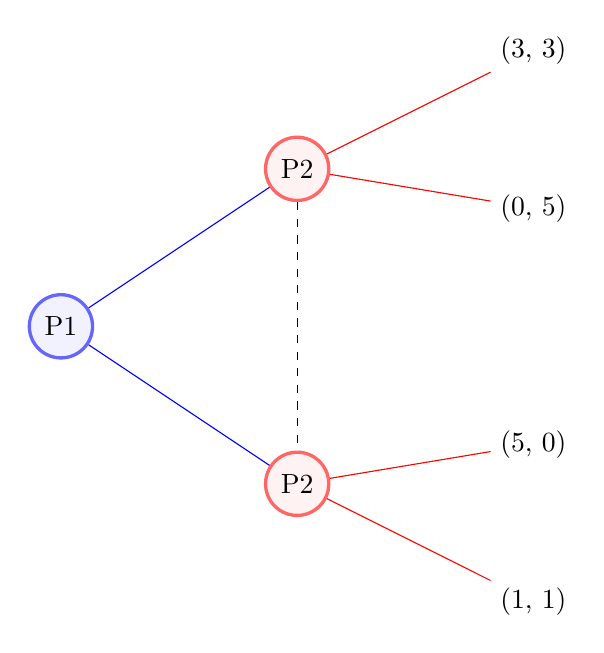
\begin{tikzpicture}
    \node[circle, draw=blue!60, fill=blue!5, very thick, minimum size=7mm] (P1) at (0, 0) {P1};
    \node[circle, draw=red!60, fill=red!5, very thick, minimum size=7mm]  (P21) at (3, 2) {P2};
    \node[circle, draw=red!60, fill=red!5, very thick, minimum size=7mm] (P22) at (3, -2) {P2};
    \draw[blue, thin] (P1) -- (P21);
    \draw[blue, thin] (P1) -- (P22);
    \node (CC) at (6, 3.5) {(3, 3)};
    \node (CD) at (6, 1.5) {(0, 5)};
    \node (DC) at (6, -1.5) {(5, 0)};
    \node (DD) at (6, -3.5) {(1, 1)};
    \draw[red, thin] (P21) -- (CC);
    \draw[red, thin] (P21) -- (CD);
    \draw[red, thin] (P22) -- (DC);
    \draw[red, thin] (P22) -- (DD);
    \draw[black, dashed] (P21) -- (P22);
\end{tikzpicture}
    \caption{The extensive form representation of the PD.}\label{fig:PD_game_tree}
\end{figure}

\begin{definition}
According to~\cite{Webb2007}, a \textit{subgame} is a sub-graph of the game tree
such that:
\begin{itemize}
    \item The sub-graph begins at a decision node, say \(x_{i}\);
    \item This node, \(x_{i}\), is the only element contained in its information
    set; and
    \item The sub-graph contains all of the decision nodes which follow \(x_{i}\).
\end{itemize}   
\end{definition}

This leads to the following definition of \textit{subgame perfect equilibria},
also adapted from~\cite{Webb2007}.

\begin{definition}
    A \textit{subgame perfect equilibrium} is a Nash equilibrium which satisfies
    the condition that the strategies played define a Nash equilibrium in every
    subgame.
\end{definition}

Hence the strategy defined in Theorem~\ref{thm:seq_of_stage_NE} is a subgame
perfect equilibrium. A few final definitions are now highlighted before
introducing the Folk Theorem.

\subsubsection{Final Definitions Needed}\label{subsubsec:Final_Defs_Needed}
Now, in order to be able to discuss the payoffs of strategies in infinite games,
a few final definitions are required.

\begin{definition}\label{def:disc_payoff}
In~\cite{Knight2017} a \textit{discounted payoff} is defined as:
\begin{equation}
    V_{i}(\sigma) = \sum_{t=1}^{\infty}{\delta^{t-1}U_{i}(\sigma)},
\end{equation}
where the discount factor, \(\delta \), can be thought of as the probability
that the game continues. That is, the probability that another stage game will
be played. 
\end{definition}

Definition~\ref{def:disc_payoff} can be used to define \textit{average payoffs}.

\begin{definition}
    According to~\cite{Knight2017}, the \textit{average payoffs} per stage
    game, are given by:
   \begin{equation}
        \frac{1}{\overline{T}}V_{i}(\sigma) = (1-\delta)V_{i}(\sigma),    
    \end{equation}
    where \(\overline{T} = \frac{1}{1-\delta}\) is the average length of a game. 
\end{definition}

Finally, Figure~\ref{fig:Feasible_Payoff_Plot} shows those payoffs which are
individually rational for a two player version of PD\@. In
general, an \textit{individually rational payoff} is an average payoff which
exceeds those obtained in the stage Nash equilibria for all
players~\cite{Knight2017}. Often the Nash equilibrium payoff is not the
optimal payoff players could achieve.

\begin{figure}
    \centering
    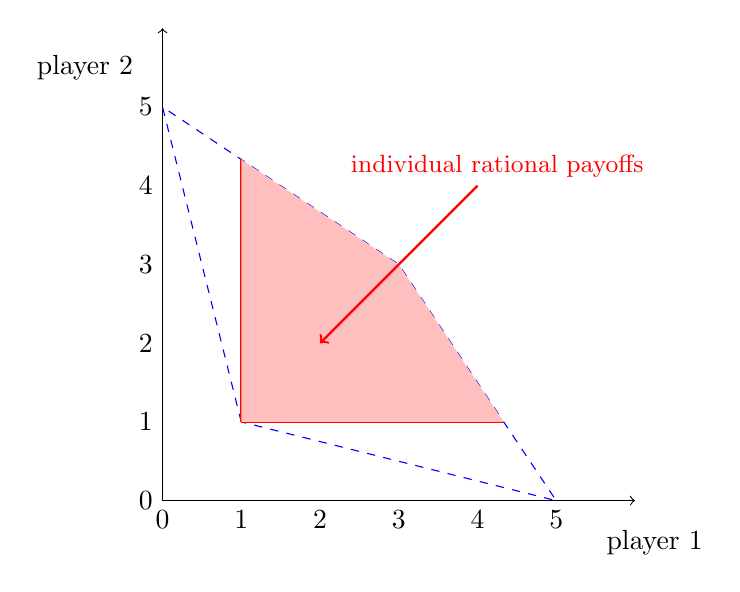
\begin{tikzpicture}
    \draw[->] (0,0) -- (6,0);
    \node[below] at (6.25, -0.25) {player 1};
    \draw[->] (0,0) -- (0,6);
    \node[left] at (-0.25, 5.5) {player 2};
    \foreach \x/\xtext in {0,1,2,3,4,5}
        \node[below] at (\x, 0) {$\xtext$};
    \foreach \y/\ytext in {0,1,2,3,4,5}
        \node[left] at (0, \y) {$\ytext$};
    \draw[blue, dashed] (1,1) -- (0,5) -- (3,3) -- (5,0) -- (1,1);
    \draw[red, thick] (1, 1) -- (1, 13/3);
    \draw[red, thick] (1, 1) -- (13/3, 1);
    \fill[red!25] (1, 1) -- (1, 13/3) -- (3, 3) -- (13/3, 1) -- (1, 1);
    \node[red] at (4.25, 4.25) {\small individual rational payoffs};
    \draw[red, ->, thick] (4, 4) -- (2, 2);
\end{tikzpicture}
    \caption{A plot highlighting the individually rational payoffs for the PD.}\label{fig:Feasible_Payoff_Plot}
\end{figure}

\section{Folk Theorem}\label{sec:Folk_Thm}
This section contains the statement and proof of the main theorem in this project.

According to~\cite{Webb2007}, the Folk Theorems are
so-called because their results were well-known before a formal proof was
provided. In general, these theorems state that players can achieve a better
payoff than the Nash equilibrium (if the Nash equilibrium payoff is not optimal)
when the stage game is repeated many times and the probability of the game
continuing is high enough. 

It is believed that~\cite{Friedman1971} was one of the
first to provide a formal proof to the widely accepted Folk
Theorem~\cite{Abreu1994, Webb2007}. Thus, the presentation of the statement and
proof given here is adapted from~\cite{Friedman1971} as well as~\cite{Knight2017}.

\begin{theorem}\label{thm:Folk}
    Assume the conditions provided in Section~\ref{subsec:Assumptions} are
    satisfied for the given infinite repeated game. Then, for any individually
    rational payoff \(V_{i}\), there exists a discount parameter \(\delta^{*}\)
    such that for all \(\delta_{i}\), \(0 < \delta^{*} < \delta_{i} < 1\) there
    is a subgame perfect Nash equilibria with payoffs equal to \(V_{i}\).
\end{theorem}

\subsection{Assumptions}\label{subsec:Assumptions}
Here, the assumptions which Friedman~\cite{Friedman1971} requires the
infinite repeated game to satisfy in order for Theorem~\ref{thm:Folk} to hold are listed.
\begin{enumerate}
    \item The mixed action sets, \(\Sigma_{i}\) are compact and convex for all
    \(i\in N\). 

    \item The payoff functions, \(U_{i}: \Sigma \to \mathbb{R}\), are continuous
    and bounded for all \(i\in N\).

    \item The \(U_{i}(\sigma)\)s are quasi-concave\footnote{According
    to~\cite{Stover}, a real-valued function \(f\), defined on a convex subset
    \(C \subset \mathbb{R}^n\), is \textit{quasi-concave} if for all \(\alpha
    \in \mathbb{R}\), the set \( \{ x \in C : f(x) \ge a \} \) is convex.}
    functions of \(sigma_{i}\) for all \(i\in N\).

    \item If  \(U_{i}^{\prime} \le U_{i}^{\prime\prime}\), for all \(i\in N\)
    and \(U_{i}^{\prime}, U_{i}^{\prime\prime} \in \mathcal{U}\), then, for all
    \(U_{i}^{\prime} \le U \le U_{i}^{\prime\prime}\), \(U \in \mathcal{U}\). Here, \(\mathcal{U}\)
    is defined to be the set of feasible payoffs, \( \{ U(\sigma) : \sigma \in
    \Sigma \} \), where \(U(\sigma) = (U_{1}(\sigma), U_{2}(\sigma), \ldots,
    U_{N}(\sigma))\).

    \item \(\mathcal{U}^{*}\) is concave, where \(\mathcal{U}^{*} \subset \mathcal{U}\) denotes the
    set of all Pareto optimal payoffs\footnote{The paper~\cite{Friedman1971} defines a
    \textit{Pareto optimal payoff} as a point in the payoff space
    \(U_{i}(\sigma^{*})\) which satisfies the conditions: \(\sigma^{*} \in
    \Sigma \) and \(U_{i}(\sigma^{*}) > U_{i}(\sigma)\) for all \(i \in N\)}.

    \item All stage games are identical in the infinitely repeated game.

    \item The discount parameter, \(\delta \), is equal in all time periods.
    
    \item The stage game has a unique Nash equilibrium.

    \item The Nash equilibrium is not Pareto optimal\footnote{That is, the
    payoff yielded from the Nash equilibrium is not a Pareto optimal payoff.}. 
\end{enumerate}

Note~\cite{Friedman1971} later goes on to prove that assumptions
six to nine can be removed with only a small effect on the result. However,
since the game being studied in this project is the IPD (which satisfies
all the above assumptions), this generalisation will be omitted. Only the
proof of the original theorem will be provided.

\subsection{Proof of the Folk Theorem}

\begin{proof}
    Consider the set of all actions which yield greater payoffs than the Nash
    equilibrium, denoted by:
    \begin{equation}
        B = \{\sigma : \sigma \in \Sigma, U_{i}(\sigma) > U_{i}(\sigma^{*}), i \in N\}
    \end{equation}
    where \(\sigma^{*}\) is the Nash equilibrium strategy. Define the following trigger strategy:
    \begin{equation}\label{eqn:trigger_strategy}
        \sigma_{i1} = \sigma_{i}^{\prime};~~~
        \sigma_{it} = \begin{cases}
            \sigma_{i}^{\prime}, & \quad \text{if } \sigma_{j\tau}=\sigma_{j}^{\prime} \ j \ne i, \tau=1, 2, \ldots, t-1, t=2, 3, \ldots \\
            \sigma_{i}^{*}, & \quad \text{otherwise},
        \end{cases}
    \end{equation}
    where \(\sigma_{i}^{\prime} \in B\). In words, the \(i\)th player will choose \(\sigma_{i}^{\prime}\) unless any
    other player does not play \( \sigma_{j}^{\prime}\), in which case they
    continue by playing their Nash equilibrium action, \(\sigma_{i}^{*}\). 
    
    Now, by definition, the strategy in~(\ref{eqn:trigger_strategy}) is an
    equilibrium of the repeated game if 
    \begin{equation}
        \sum_{\tau=0}^{\infty}{\delta_{i}^{\tau}U_{i}(\sigma_{i}^{\prime})} > U_{i}(\sigma_{-i}^{\prime}, t_{i}) + \sum_{\tau=1}^{\infty}{\delta_{i}^{\tau}U_{i}(\sigma^{*})},~~~ i \in N,
    \end{equation}
    which can be rearranged to 
    \begin{equation}
        \frac{\delta_{i}}{1-\delta_{i}}[U_{i}(\sigma^{\prime}) - U_{i}(\sigma^{*})] > U_{i}(\sigma_{-i}^{\prime}, t_{i}) - U_{i}(\sigma{\prime}),~~~ i \in N,
    \end{equation}
    where \(U_{i}(\sigma_{-i}^{\prime}, t_{i}) = \max_{\sigma_{i} \in
    \Sigma_{i}}{U_{i}(\sigma_{-i}^{\prime}, \sigma_{i})}\), \(t_{i} \in
    \Sigma_{i}\). Note, \(\sigma_{-i} = (\sigma_{1}, \ldots, \sigma_{i-1},
    \sigma_{i+1}, \ldots, \sigma_{n})\) is the strategy vector with the \(i\)th
    player removed.

    To check if this strategy is indeed a best response to all others players,
    who are executing the same strategy in~(\ref{eqn:trigger_strategy}),
    consider their alternatives. The \(i\)th player has two options. Either
    they execute the strategy~(\ref{eqn:trigger_strategy}), or they play the
    strategy in which \(\sigma_{i1} = t_{i}\). The latter implies \(\sigma_{i\tau} =
    \sigma^{*}\) will be the best response as every other player will convert
    to \(\sigma_{j\tau} = \sigma^{*}\), for all \(\tau > 1\). Note that any
    other strategy is weakly dominated by one of these two, since playing
    \(t_{i}\) in any other stage \(\tau \ne 1\) will yield less gains due to increased discounting.

    Now if, from playing the Nash equilibria, the discounted loss 
    \begin{equation}\label{eqn:discounted_loss}
        \frac{\delta_{i}}{1-\delta_{i}}[U_{i}(\sigma^{\prime}) -
        U_{i}(\sigma^{*})],
    \end{equation}
    is greater than the gain achieved by playing
    \(t_{i}\) against \(\sigma_{-i}^{\prime}\), then the rational
    strategy choice for player \(i\), assuming all other players are
    executing~(\ref{eqn:trigger_strategy}), is to play~(\ref{eqn:trigger_strategy}).
    
    Observe, as the discount parameter, \(\delta \to 1\) from
    below, the discounted loss in~(\ref{eqn:discounted_loss}) tends to infinity.
    However, the gain obtained from playing \(t_{i}\), that is,
    \(U_{i}(\sigma_{-i}^{\prime}, t_{i}) - U_{i}(\sigma{\prime})\) is finite.
    Thus, for all \(\sigma_{i}^{\prime} \in B\) there exists a \(\delta^{*} \in
    (0, 1)\) such that for all \(\delta_{i} > \delta^{*}\), the
    strategy~(\ref{eqn:trigger_strategy}) is optimal against the same strategy
    for all players \(j \ne i\). Therefore, if the conditions are true for all
    players \(i = 1,2,\ldots,n\), the strategy \((\bar{\sigma}_{1},
    \bar{\sigma}_{2}, \ldots, \bar{\sigma}_{n})\), where  \(\bar{\sigma}_{i}\)
    denotes~(\ref{eqn:trigger_strategy}), yields a Nash equilibrium.

    Finally, by construction, the strategy~(\ref{eqn:trigger_strategy}) is
    indeed a subgame perfect equilibrium. 
\end{proof}


\section{Aims of the Project}\label{sec:Aims_of_the_Project}
This project stemmed from an initial idea presented in a game theory assignment
completed by the author. The topic of this coursework was Nash equilibria of
repeated games and the two graphs, as presented in Figure~\ref{fig:CW_plots}, were
obtained.

\begin{figure}
    \centering
        \begin{subfigure}{0.45\textwidth}
            \centering
            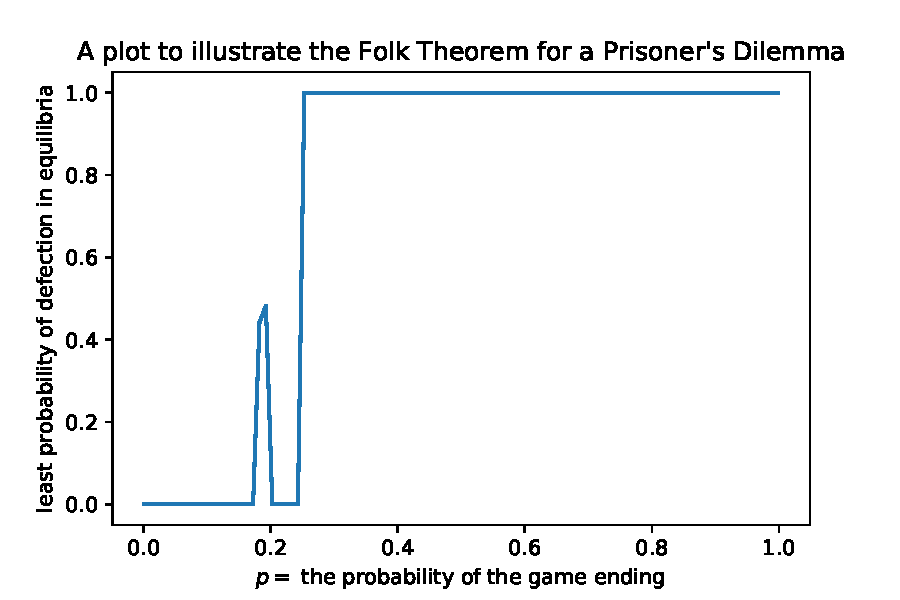
\includegraphics[width=\textwidth]{CW-graph-1.pdf}
            \caption{A plot of the least probabilities of defection against the strategies: \textit{Cooperator}, \textit{TitForTat} and \textit{Random}. Here, the \(p\)-threshold is approximately 0.25.}\label{fig:CW_graph_1}
        \end{subfigure}
        \hspace{3pt}
        \begin{subfigure}{0.45\textwidth}
            \centering
            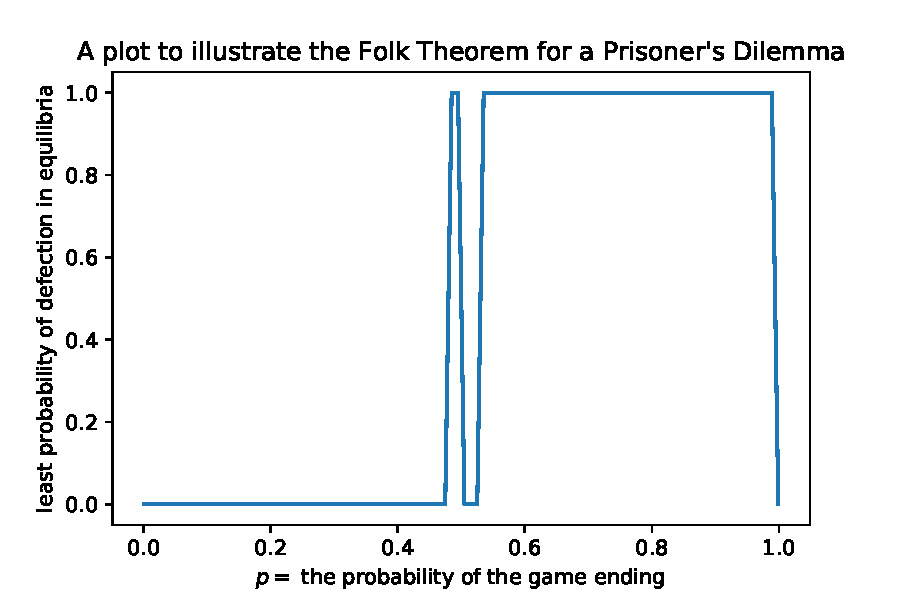
\includegraphics[width=\textwidth]{CW-graph-2.pdf}
            \caption{A plot of the least probabilities of defection against the strategies: \textit{Winner21}, \textit{AntiTitForTat} and \textit{OmegaTFT}. Here, the \(p\)-threshold is around 0.5.}\label{fig:CW_graph_2}
        \end{subfigure}
        \caption{Original plots obtained which influenced the subject of this project.}\label{fig:CW_plots}
\end{figure}

Figure~\ref{fig:CW_plots} was obtained from repeating IPD tournaments which are
implemented in Python via the package Axelrod~\cite{axelrodproject}. In general,
these tournaments are a group of strategies, who all compete in a variety of
round-robin, two-player IPDs with the aim of achieving the largest payoffs. The
implementation in Axelrod allows for the simulation and analysis of IPD
tournaments under different environments. For example:
\begin{itemize}
    \item It is possible to vary the number of strategies making the groups competing in the
    tournament\footnote{In this project, the group of strategies will be
    referred to as a \textit{player set} for clarity.
    Consider Figure~\ref{fig:CW_graph_1}, the player set here consists of the
    strategies: \textit{Cooperator}, \textit{TitForTat}, \textit{Random} and
    \textit{Defector}.}.
    
    \item Both finite and infinite IPD can be considered. The infinite IPD is
    simulated through the scenario of a probabilistic ending, denoted throughout
    this study as \(p_{e}\)\footnote{The probability of the game ending,
    \(p_{e}\), will also be referred to as a game-ending
    probability, in this project.}. Note, \(p_{e}\) is related to the discount
    parameter, \(\delta \), introduced in Definition~\ref{def:disc_payoff}, by \(p_{e}
    = 1 - \delta \).
    
    \item Varying levels of noise can be introduced. This is referred to as
    \textit{standard PD noise}\footnote{Note, there are three potential sources
    of noise within an IPD tournament. In order to differentiate between them
    the following terms are used. \textit{Standard PD noise} to refer to the
    probability of an action being altered; \textit{stochastic player noise} to
    refer to the noise induced by a stochastic strategy; and \textit{unexpected
    noise} to refer to noise which is expected from running numerical experiments.} within this report. According
    to~\cite{glynatsi2020meta}, \textit{standard PD noise} is the probability,
    \(p_{n}\), of an action being altered within any particular round. That is,
    the probability of a \(C\) being seen as a \(D\) and vice versa.
\end{itemize}

The two plots seen in Figure~\ref{fig:CW_plots} were yielded from setting \(p_{n} =
0\), the player set size equal to four, \(p_{e}\) taking 100 distinct values
within (0, 1) and each tournament to repeat 100 times. The graphs show the least
probability of defection obtained in the Nash equilibria of the corresponding
game. Note, the `corresponding game' here refers to the matrix of mean payoff
values which can be calculated from the tournament results of each strategy
(see Chapter~\ref{ch:Methods} for further explanation of this).  

From Figure~\ref{fig:CW_plots}, it can be seen that there is a clear game-ending
probability \(p_{e}\) for which the least probability of defection goes to zero.
In this project, this probability is defined as a \textit{\(p\)-threshold}.
However, what was most intriguing was that the two different games obtained had
a different \(p\)-threshold. This is approximately 0.25
for Figure~\ref{fig:CW_graph_1} but for Figure~\ref{fig:CW_graph_2} the threshold
appears at around 0.5. This initiated the idea to investigate whether there are
any specific characteristics of an IPD tournament that affect the value of the
\(p\)-threshold.

Therefore, the aims of this project are as follows:
\begin{enumerate}
\item To provide a review of past and present literature already published in
the field of folk theorems;

\item To develop a program which executes a large experiment involving
tournaments of the IPD with differing environments to obtain
graphs similar to those in Figure~\ref{fig:CW_plots}; and

\item To perform analyses on where the \(p\)-thresholds seem to lie and
whether it is affected by the change in the number of players, levels of
standard PD noise, etc.
\end{enumerate}
